\chapter*{Frequency response of RME FIREFACE UCX}
A test was made to get a view of the frequency response of the Pioneer A-616 amplifier. The Pioneer A-616 amplifier is used for all measurement in this project, and therefore the frequency response is of interest. To measure the frequency response, the function from \autoref{appendix:transfer_function} is used. The test is done with and without load, to find out if the load changes the transfer function of the amplifier.

\section*{Materials and setup}
To measure the frequency response of the Pioneer A-616 amplifier, the following materials are used:
\begin{itemize}
\item RME FIREFACE UCX (Soundcard)
\item Pioneer A-616 (amplifier)
\item MATLAB 2017b (PC - Software)
\item IRmeas_fft (software) \autoref{appendix:transfer_function}
\item SEAS 33 F-WKA mounted in an enclosed 
\item XLR speaker cable
\item Jack to phone signal cable
\item Jack to banana cable
\end{itemize}

\begin{figure}[H]
\centering
\begin{picture}(0,0)%
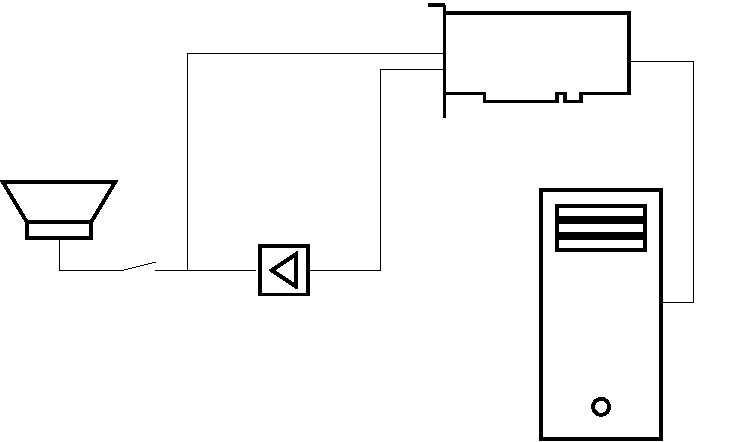
\includegraphics{pioneer_transfer_function.pdf}%
\end{picture}%
\setlength{\unitlength}{2818sp}%
%
\begingroup\makeatletter\ifx\SetFigFont\undefined%
\gdef\SetFigFont#1#2#3#4#5{%
  \reset@font\fontsize{#1}{#2pt}%
  \fontfamily{#3}\fontseries{#4}\fontshape{#5}%
  \selectfont}%
\fi\endgroup%
\begin{picture}(8338,4926)(3838,-7474)
\put(9991,-6361){Computer}%
\put(6661,-6091){Amplifier}%
\put(9271,-3211){Sound Card}%
\put(11746,-4696){USB}%
\put(8236,-3526){Out}%
\put(8281,-3031){In}%
\put(3961,-4336){Loudspeaker}%
\put(5131,-5371){Switch}%
\end{picture}%
\caption{Setup for measuring transfer function}
		\label{fig:appendix:pioneer_response}
\end{figure}

\section*{Test procedure}


\begin{enumerate}
\item The materials are set up as in \autoref{fig:appendix:pioneer_response}.
\item The signal cable is connected between the RME FIREFACE UCX output channel 1 and right Line in on the amplifier.
\item The jack to banana cable is connected between the amplifier right B output channel to the  RME FIREFACE UCX input 1 
\item The input gain of RME FIREFACE UCX at input 1 is set to \SI{20}{\decibel}
\item The output playgain is set to \SI{-18}{\decibel}
\item The input and output channel is specified in the MATLAB function "SynchronizedPlaybackAcquirer" 
\item IRmeas_fft (software) \autoref{appendix:transfer_function} is preformed with gain \SI{-40}{\decibel}, \SI{-30}{\decibel} and \SI{-27}{\decibel} of the amplifier without load 
\item then IRmeas_fft (software) \autoref{appendix:transfer_function} is preformed with gain \SI{-40}{\decibel}, \SI{-30}{\decibel} and \SI{-27}{\decibel} of the amplifier with load 
\item To be able to measure the amplifier at higher gain, the playgain is now adjusted to \SI{-35}{\decibel}
\item  IRmeas_fft (software) \autoref{appendix:transfer_function} is preformed with gain \SI{-27}{\decibel}, \SI{-16}{\decibel} and \SI{-12}{\decibel} of the amplifier without load
\item then IRmeas_fft (software) \autoref{appendix:transfer_function} is preformed with gain \SI{-27}{\decibel}, \SI{-16}{\decibel} and \SI{-12}{\decibel} of the amplifier with load
\item The measured gain from the RME FIREFACE UCX is subtracted respectively to the playgain, to get a true voltage gain of the amplifier.
\item The transfer function is plotted from \SI{20}{\hertz} to \SI{20}{\kilo\hertz} for every measurement.

\end{enumerate}

\section*{Results}



On \autoref{fig:appendix:rme_response_result} it is seen that the soundcard only have a non linearity of \SI{0.26}{\decibel} from \SI{20}{\hertz} to \SI{20}{\kilo\hertz} between output data and input data. 

\begin{figure}[H]
	\centering
	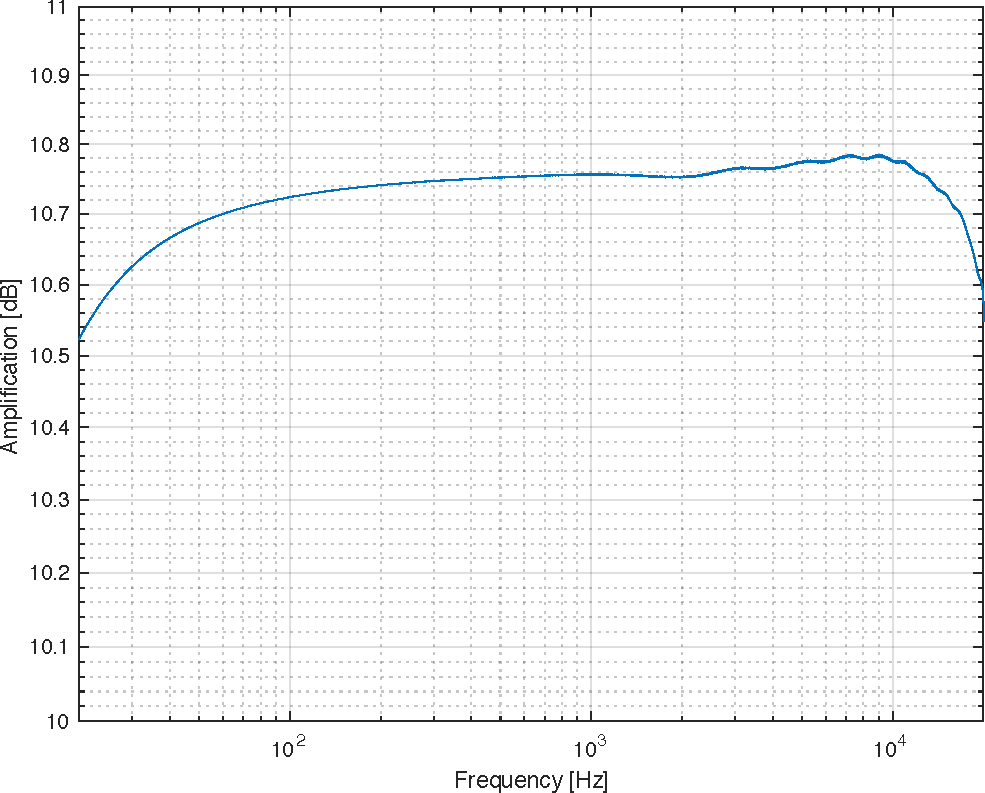
\includegraphics[width=1\textwidth]{RME_FIREFACE_UCX_tf.pdf}
	\caption{The frequency response of the RME FIREFACE UCX with input sensitivity at 20}
		\label{fig:appendix:rme_response_result}
\end{figure}

